% A LaTeX template for EXECUTIVE SUMMARY of the MSc Thesis submissions to 
% Politecnico di Milano (PoliMi) - School of Industrial and Information Engineering
%
% S. Bonetti, A. Gruttadauria, G. Mescolini, A. Zingaro
% e-mail: template-tesi-ingind@polimi.it
%
% Last Revision: October 2021
%
% Copyright 2021 Politecnico di Milano, Italy. NC-BY

\documentclass[11pt,a4paper,twocolumn]{article}

%------------------------------------------------------------------------------
%	REQUIRED PACKAGES AND  CONFIGURATIONS
%------------------------------------------------------------------------------
% PACKAGES FOR TITLES
\usepackage{titlesec}
\usepackage{color}

% PACKAGES FOR LANGUAGE AND FONT
\usepackage[utf8]{inputenc}
\usepackage[english]{babel}
\usepackage[T1]{fontenc} % Font encoding

% PACKAGES FOR IMAGES
\usepackage{graphicx}
\graphicspath{{Images/}{../LaTex_Project/imgs/}{../UP-MAVT/results/pdfs/}{../UP-MAVT/elicitation_results/plots/}} % Path for images' folder
\usepackage{eso-pic} % For the background picture on the title page
\usepackage{subfig} % Numbered and caption subfigures using \subfloat
\usepackage{caption} % Coloured captions
\usepackage{transparent}

% STANDARD MATH PACKAGES
\usepackage{amsmath}
\usepackage{amsthm}
\usepackage{bm}
\usepackage[overload]{empheq}  % For braced-style systems of equations

% PACKAGES FOR TABLES
\usepackage{tabularx}
\usepackage{longtable} % tables that can span several pages
\usepackage{colortbl}

% PACKAGES FOR ALGORITHMS (PSEUDO-CODE)
\usepackage{algorithm}
\usepackage{algorithmic}

% PACKAGES FOR REFERENCES & BIBLIOGRAPHY
\usepackage[colorlinks=true,linkcolor=black,anchorcolor=black,citecolor=black,filecolor=black,menucolor=black,runcolor=black,urlcolor=black]{hyperref} % Adds clickable links at references
\usepackage{cleveref}
\usepackage[square, numbers, sort&compress]{natbib} % Square brackets, citing references with numbers, citations sorted by appearance in the text and compressed
\bibliographystyle{plain} % You may use a different style adapted to your field

% PACKAGES FOR THE APPENDIX
\usepackage{appendix}

% PACKAGES FOR ITEMIZE & ENUMERATES 
\usepackage{enumitem}

% OTHER PACKAGES
\usepackage{amsthm,thmtools,xcolor} % Coloured "Theorem"
\usepackage{comment} % Comment part of code
\usepackage{fancyhdr} % Fancy headers and footers
\usepackage{lipsum} % Insert dummy text
\usepackage{tcolorbox} % Create coloured boxes (e.g. the one for the key-words)
\usepackage{stfloats} % Correct position of the tables

%-------------------------------------------------------------------------
%	NEW COMMANDS DEFINED
%-------------------------------------------------------------------------
% EXAMPLES OF NEW COMMANDS -> here you see how to define new commands
\newcommand{\bea}{\begin{eqnarray}} % Shortcut for equation arrays
\newcommand{\eea}{\end{eqnarray}}
\newcommand{\e}[1]{\times 10^{#1}}  % Powers of 10 notation
\newcommand{\mathbbm}[1]{\text{\usefont{U}{bbm}{m}{n}#1}} % From mathbbm.sty
\newcommand{\pdev}[2]{\frac{\partial#1}{\partial#2}}
% NB: you can also override some existing commands with the keyword \renewcommand

%----------------------------------------------------------------------------
%	ADD YOUR PACKAGES (be careful of package interaction)
%----------------------------------------------------------------------------


%----------------------------------------------------------------------------
%	ADD YOUR DEFINITIONS AND COMMANDS (be careful of existing commands)
%----------------------------------------------------------------------------


% Do not change Configuration_files/config.tex file unless you really know what you are doing. 
% This file ends the configuration procedures (e.g. customizing commands, definition of new commands)
\input{Configuration_files/config}

% Insert here the info that will be displayed into your Title page 
% -> title of your work
\renewcommand{\title}{Evaluating Nuclear Reactor Designs for Deployment in Europe}
% Subtitle: added for executive summary
\newcommand{\subtitle}{A Multi-Criteria Decision Support Framework with Uncertainty Propagation}
% -> author name and surname
\renewcommand{\author}{Simone Pagliuca}
% -> MSc course
\newcommand{\course}{Nuclear Engineering - Ingegneria Nucleare}
% -> advisor name and surname
\newcommand{\advisor}{Prof. Stefano Lorenzi}
% IF AND ONLY IF you need to modify the co-supervisors you also have to modify the file Configuration_files/title_page.tex (ONLY where it is marked)
\newcommand{\firstcoadvisor}{Prof. Russell McKenna}
\newcommand{\firstcoadvisoraffil}{ETH-Zurich}
\newcommand{\secondcoadvisor}{Dr. Peter Burgherr}
\newcommand{\secondcoadvisoraffil}{Paul Scherrer Institute (PSI)}
\newcommand{\thirdcoadvisor}{Dr. Huang He}
\newcommand{\thirdcoadvisoraffil}{Paul Scherrer Institute (PSI)}
% -> academic year
\newcommand{\YEAR}{2025-2026}

%-------------------------------------------------------------------------
%	BEGIN OF YOUR DOCUMENT
%-------------------------------------------------------------------------
\begin{document}

%-----------------------------------------------------------------------------
% TITLE PAGE
%-----------------------------------------------------------------------------
% Do not change Configuration_files/TitlePage.tex (Modify it IF AND ONLY IF you need to add or delete the Co-advisors)
% This file creates the Title Page of the document
% DO NOT REMOVE SPACES BETWEEN LINES!

\twocolumn[{\begin{@twocolumnfalse}

\AddToShipoutPicture*{\BackgroundPic}

\hspace{-0.6cm}
\includegraphics[width=0.6\textwidth]{logo_polimi_ing_indinf.eps}

\vspace{-1mm}
\fontsize{0.3cm}{0.5cm}\selectfont \bfseries \textsc{\color{bluePoli} Executive Summary of the Thesis}\\

\vspace{-0.2cm}
\Large{\textbf{\color{bluePoli}{\title}}}\\
\vspace{2pt}
{\large\textbf{\color{bluePoli}\subtitle}}\\

\vspace{-0.2cm}
\fontsize{0.3cm}{0.5cm}\selectfont \bfseries \textsc{\color{bluePoli} Laurea Magistrale in \course}\\

\vspace{-0.2cm}
\fontsize{0.3cm}{0.5cm} \selectfont \bfseries Author: \textsc{\textbf{\author}}\\

\vspace{-0.4cm}
\fontsize{0.3cm}{0.5cm}\selectfont \bfseries Advisor: \textsc{\textbf{\advisor}}\\

% if only ONE co-advisor is present:
%\vspace{-0.4cm}
%\fontsize{0.3cm}{0.5cm}\selectfont \bfseries Co-advisor: \textsc{\textbf{\firstcoadvisor}}\\
% if more than one co-advisors are present:
\vspace{-0.4cm}
\fontsize{0.3cm}{0.5cm}\selectfont \bfseries Co-advisors: \textsc{\textbf{\firstcoadvisor}}\textsuperscript{1}, \textsc{\textbf{\secondcoadvisor}}\textsuperscript{2}, \textsc{\textbf{\thirdcoadvisor}}\textsuperscript{2}\\

\vspace{-0.4cm}
\fontsize{0.3cm}{0.5cm}\selectfont \bfseries Academic year: \textsc{\textbf{\YEAR}}

\vspace{4pt}
{\small\itshape\noindent\textsuperscript{1}\firstcoadvisoraffil\quad\textsuperscript{2}\secondcoadvisoraffil}

\small \normalfont

\vspace{11pt}

\centerline{\rule{1.0\textwidth}{0.4pt}}

\vspace{15pt}
\end{@twocolumnfalse}}]

\thispagestyle{plain} % In order to not show the header in the first page

%%%%%%%%%%%%%%%%%%%%%%%%%%%%%%
%%     THESIS MAIN TEXT     %%
%%%%%%%%%%%%%%%%%%%%%%%%%%%%%%

%-----------------------------------------------------------------------------
% INTRODUCTION
%-----------------------------------------------------------------------------
\section{Introduction}
\label{sec:introduction}
The European energy sector is at a crossroads, reshaped by the imperatives of decarbonization and energy security. Recent disruptions, such as the COVID-19 pandemic, the Russian invasion of Ukraine, and accelerated climate targets, have forced policymakers to reconsider the role of nuclear power as a mean to overcome these challenges. Among all evidence of this shift, the most significant is the EU’s inclusion of nuclear power in its taxonomy of sustainable economic activities \cite{EUTaxonomy}.

The commitment to reactor design for deployment requires balancing technical, economic, regulatory, and social trade-offs, knowing the decision taken today will have consequences for decades, policymakers are likely to seek help from decision support systems. Yet such analyses are inherently uncertain: limited data, reliance on projections, and subjective preference weightings introduce ambiguity. Without systematic treatment, this uncertainty risks compromising the transparency and robustness of policy support tools undermining its usefulness.

Although the importance of addressing uncertainty is widely recognized in Multi-Criteria Decision Analysis (MCDA), few studies propagate it comprehensively. Most reduce it to static ranges or confidence intervals rather than leveraging full probability distributions. Moreover, no open-source frameworks currently exist for this purpose, limiting reproducibility and transparency. To address this research gap, this thesis presents UP-MAVT (Uncertainty Propagated Multi-Attribute Value Theory), a framework that propagates all uncertain variables in a MAVT framework. 

The method is then applied to a case study designed to fill another literature gap: while MCDA studies on nuclear power are common, they typically focus either on site selection problems or technology assessment (e.g. Solar vs Nuclear or HTGR vs MSR). Therefore, there is no study that compares specific reactor models within a well-defined decision context. In this thesis we evaluate six reactor designs across four European countries (Italy, France, Poland, and Switzerland), adopting the perspective of governmental energy planners targeting deployments in the mid-2030s.



%-----------------------------------------------------------------------------
% METHODOLOGY
%-----------------------------------------------------------------------------
\section{Methodology}
\label{sec:methodology}

\subsection{Multi-Attribute Value Theory}
This analysis adopts Multi-Attribute Value Theory (MAVT), a preference-modelling framework introduced by Keeney~\cite{KEENEY1996537} that quantifies decision-makers’ values through functions $v_j(x)$, which are able to capture non-linear relationships between indicator values and their perceived worth. To address uncertainty in preference elicitation, experts self-assessed their confidence on a 0–4 scale, which was used to introduce controlled deviations around the elicited points. The simple mathematical structure and transparency~\cite{SCHUWIRTH2012472} of the MAVT framework was deemed well suited for the methodological extension proposed in this work.

\subsection{PILE-BWT Method for Weight Elicitation}
Expert elicitation of the importance weights $w_j$, a state-of-the-art method called PILE-BWT (Pivot-Linked Elicitation for Hierarchical Best-Worst Tradeoff)~\cite{Huang2026} was employed. This approach provides uncertainty ranges for each criteria weight, making it particularly suitable for the UP-MAVT framework. 

\subsection{Qualitative Indicators}
Of the 15 indicators in the case study, five were qualitative and required expert assessment. A novel elicitation procedure was designed: experts first ranked the alternatives, then adjusted the value functions to reflect differences between tiers in the ranking. As with quantitative indicators, they self-assessed their confidence on a 0–4 scale, introducing controlled deviations to quantify uncertainty in these qualitative judgments. This approach was well received by experts, who appreciated the intuitiveness of the method and the ability to express uncertainty in their judgments.

\subsection{Uncertainty Propagation Framework}
The novel UP-MAVT framework replaces deterministic inputs with probabilistic representations, treating criterion data, value functions, and weights as distributions and propagating them to output distributions. Unlike prior studies (e.g., \cite{Ezbakhe2018}) that relied on summary statistics, this method leverages the information of complete distributions. The generalized formulation is given by:

\begin{multline}
\text{PDF}_{A_i}(a) = \sum_{j=1}^N \iiint \delta\left(a - v_j(x_{ij})w_j\right) \\
\cdot \text{PDF}_X \cdot \text{PDF}_V \cdot \text{PDF}_W \, dx \, dv \, dw
\label{eq:mavt_up}
\end{multline}

In practice, the propagation is achieved by Monte Carlo simulation, to this goal two complementary approaches are employed: Strict Monte Carlo (SMC) which preserves each expert's opinion as independent, serving as a consensus diagnostic tool; and Non-Strict Monte Carlo (NSMC) which samples from all possible opinions, generating conservative aggregate probabilistic rankings. The framework supports both fully compensatory (weighted sum) and partially compensatory (geometric mean, harmonic mean) aggregation methods to accommodate different compensation philosophies.

The UP-MAVT workflow (Figure~\ref{fig:workflow}) illustrates the sources of uncertainties from criterion data, value functions, and weights and how they are propagated through the Monte Carlo code though the two methods.

\subsection{Elicitation Support Tools}
A suite of graphical tools was developed to assist experts across all elicitation stages: value functions, qualitative indicators, and weights. Designed to reduce practitioner burden, improve transparency, and enhance engagement, these tools also cut elicitation time while raising data quality. Experts praised their intuitiveness and effectiveness in capturing judgments. The tools will be released publicly alongside the UP-MAVT codebase to support broader adoption.

%-----------------------------------------------------------------------------
% CASE STUDY
%-----------------------------------------------------------------------------
\section{Case Study Design}
\label{sec:case_study}

The analysis compares six light-water reactor designs, three Generation~III+ and three SMRs, across four European countries deliberately selected to capture a wide range of energy scenarios:

\begin{itemize}
    \item {Italy}: no operational nuclear fleet, high import dependence ($\sim$30\% of demand), currently exploring reintroduction.
    \item {Poland}: strong public support for nuclear, 55\% coal-based generation, highest GHG emission intensity in Europe.
    \item {Switzerland}: uncertain public support, low demand, generation dominated by renewables (65\%).
    \item {France}: 67\% nuclear share in generation, established industrial base.
\end{itemize}

The selection of reactor designs was determined from systematic screening of the IAEA PRIS and ARIS databases, excluding designs from non-allied suppliers (Russia, China, India), non-commercial or regulatory-lagging designs, and prototypes. Table~\ref{tab:reactors} summarizes the final selection.

\begin{table}[H]
\centering
\caption{Selected reactor designs for analysis.}
\label{tab:reactors}
\begin{tabular}{ll}
\hline
\rowcolor{bluePoli!40}
{Reactor} & {Supplier} \T\B \\
\hline \hline
APR-1400 & KEPCO (S.Korea) \T\B \\
EPR-1750 & Framatome (France) \T\B \\
AP1000 & Westinghouse (USA) \T\B \\
BWRX-300 & GE Vernova (USA) \T\B \\
RR SMR & Rolls-Royce (UK) \T\B \\
NuScale & NuScale Power (USA) \B \\
\hline
\end{tabular}
\end{table}

The 15~indicators span four groups: \textit{Technical} (thermal efficiency, discharge burnup, net power output, load following capabilities), \textit{Feasibility} (design maturity, licensing status, supplier availability), \textit{Economic} (capital investment, design/construction complexity, operative costs), and \textit{Social} (electricity market benefit, GHG reduction, perceived safety, nuclear waste).

A total of nine experts in the nuclear domain participated in the elicitation process. Four performed ``full elicitation'' (value functions, qualitative indicators, and weights); while the remaining five experts participated in abbreviated sessions focused only on the assessment of  qualitative indicator. The panel covered risk assessment, nuclear safety, energy system modelling, plant operations, construction, and project management, with experience ranging from PhD students to senior scientists and industry veterans with over 20~years of experience.

%-----------------------------------------------------------------------------
% RESULTS
%-----------------------------------------------------------------------------
\section{Results and Discussion}
\label{sec:results}

Results were aggregated using three methods: weighted sum (fully compensatory), geometric mean, and harmonic mean (partially compensatory). The geometric mean was selected for final interpretation as it penalizes poor performance the in heavily weighted criteria the most among the three methods, aligning more closely with opinions expressed by experts during interviews.

\subsection{Dominance of Large Reactors}

A striking and robust result emerged: large reactor designs consistently outperformed SMRs across all four countries, all expert assessments, and all aggregation methods. Contrary to initial expectations, even in Switzerland, where smaller designs were expected to better match the low grid demand, all experts preferred large-scale solutions. Multiple experts argued that nuclear power's primary value lies in its role as a stable, large-scale baseload source for national energy strategies, even at the expense of flexibility. Experts suggested that SMRs may find more suitable applications in private-sector contexts (industrial process heat, remote energy systems) rather than central grid integration. The observed dominance of large reactors was also driven by their advantages in licensing readiness, supplier availability, and proven ground, all of which favour established designs over SMRs technologies which lack substantial operational demonstration.

\begin{figure}[htbp]
    \centering
    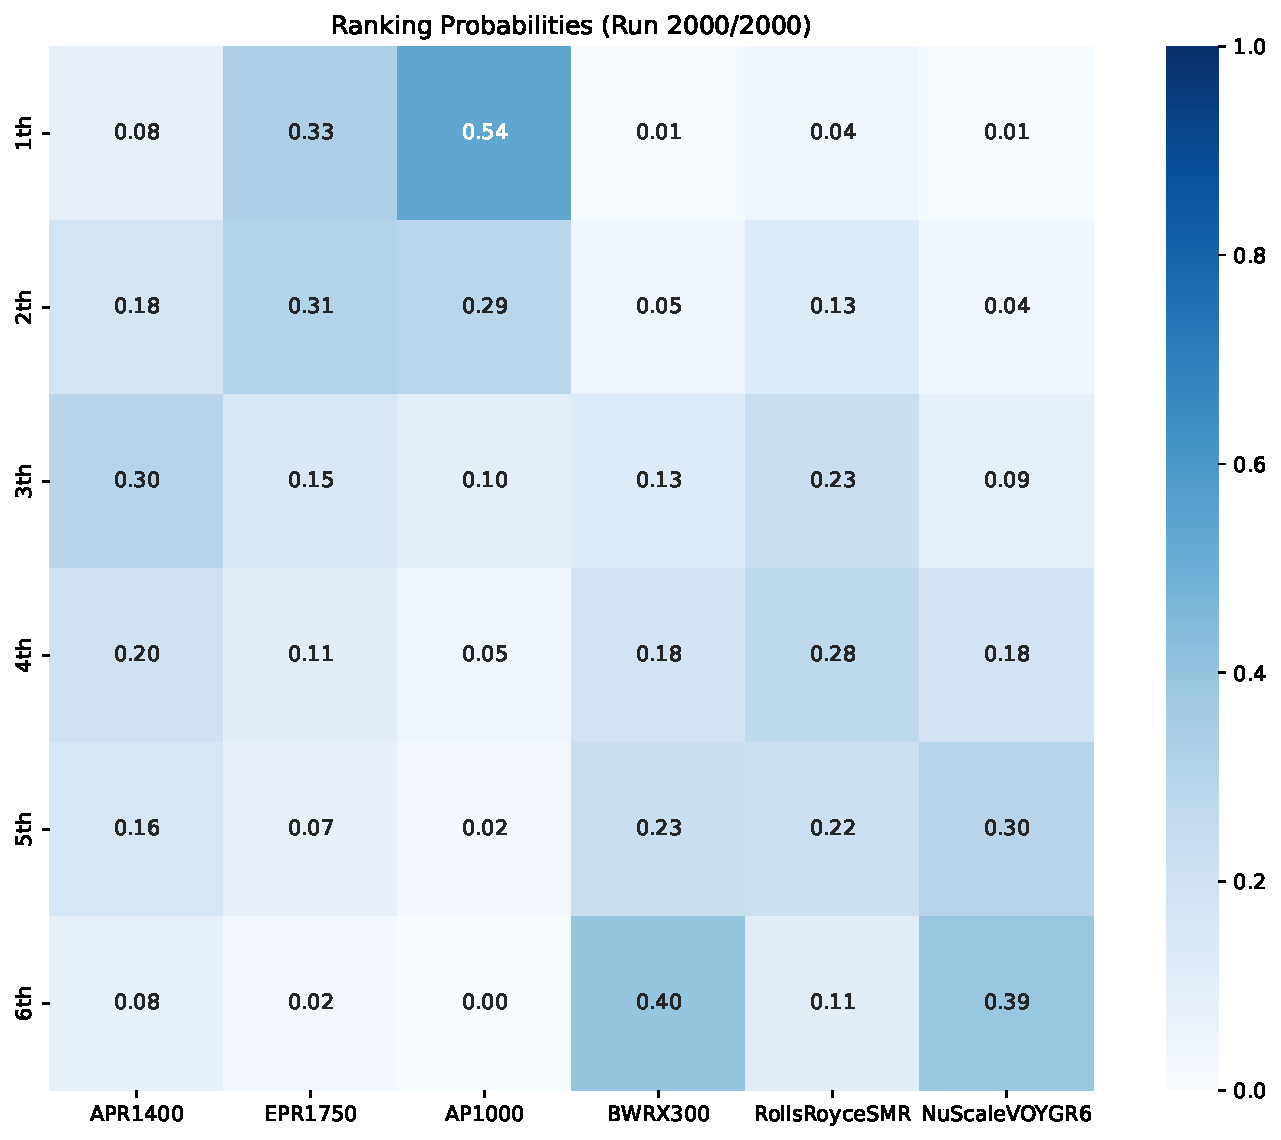
\includegraphics[width=0.95\linewidth]{Phase3_AllMethods_IT_geometric_mean_20260127_171336_heatmap.pdf}
    \caption{NSMC ranking heatmap for Italy (geometric mean). Each column represents an alternative and each row a tier in the ranking; darker cells indicate higher probability of an alternative achieving that rank. Large reactors dominate the top positions.}
    \label{fig:nsmc_italy}
\end{figure}


\subsection{Regional Patterns and Technology Rankings}

Among large reactors, the EPR and AP1000 competed for first and second place, with rank order sensitive to the aggregation method. Table~\ref{tab:modal_rankings} summarizes the modal rankings for Italy under different aggregation approaches. Under fully compensatory aggregation, the EPR secured first position due to strong technical performance (e.g. efficiency and discharge burnup), but dropped to second under partially compensatory methods where the AP1000's more balanced profile prevailed. The APR-1400 consistently ranked third, primarily due to perceived deployment challenges in the European context, including political barriers, divergent safety standards, and supply chain integration difficulties.

\begin{table}[htbp]
\centering
\caption{Modal rankings for Italy (NSMC 10,000 iterations).}
\label{tab:modal_rankings}
\begin{tabular}{lccc}
\hline
\rowcolor{bluePoli!40}
{Alternative} & {W. Sum} & {Geo.} & {Har.} \T\B \\
\hline \hline
EPR-1750       & 1 & 2 & 2 \T\B \\
AP1000         & 2 & 1 & 1 \T\B \\
APR-1400       & 3 & 3 & 3 \T\B \\
Rolls-Royce SMR & 4 & 3 & 4 \T\B \\
BWRX-300       & 6 & 5 & 6 \T\B \\
NuScale        & 5 & 6 & 5 \B \\
\hline
\end{tabular}
\end{table}

\begin{figure}[H]
	\centering
	\subfloat[Switzerland]{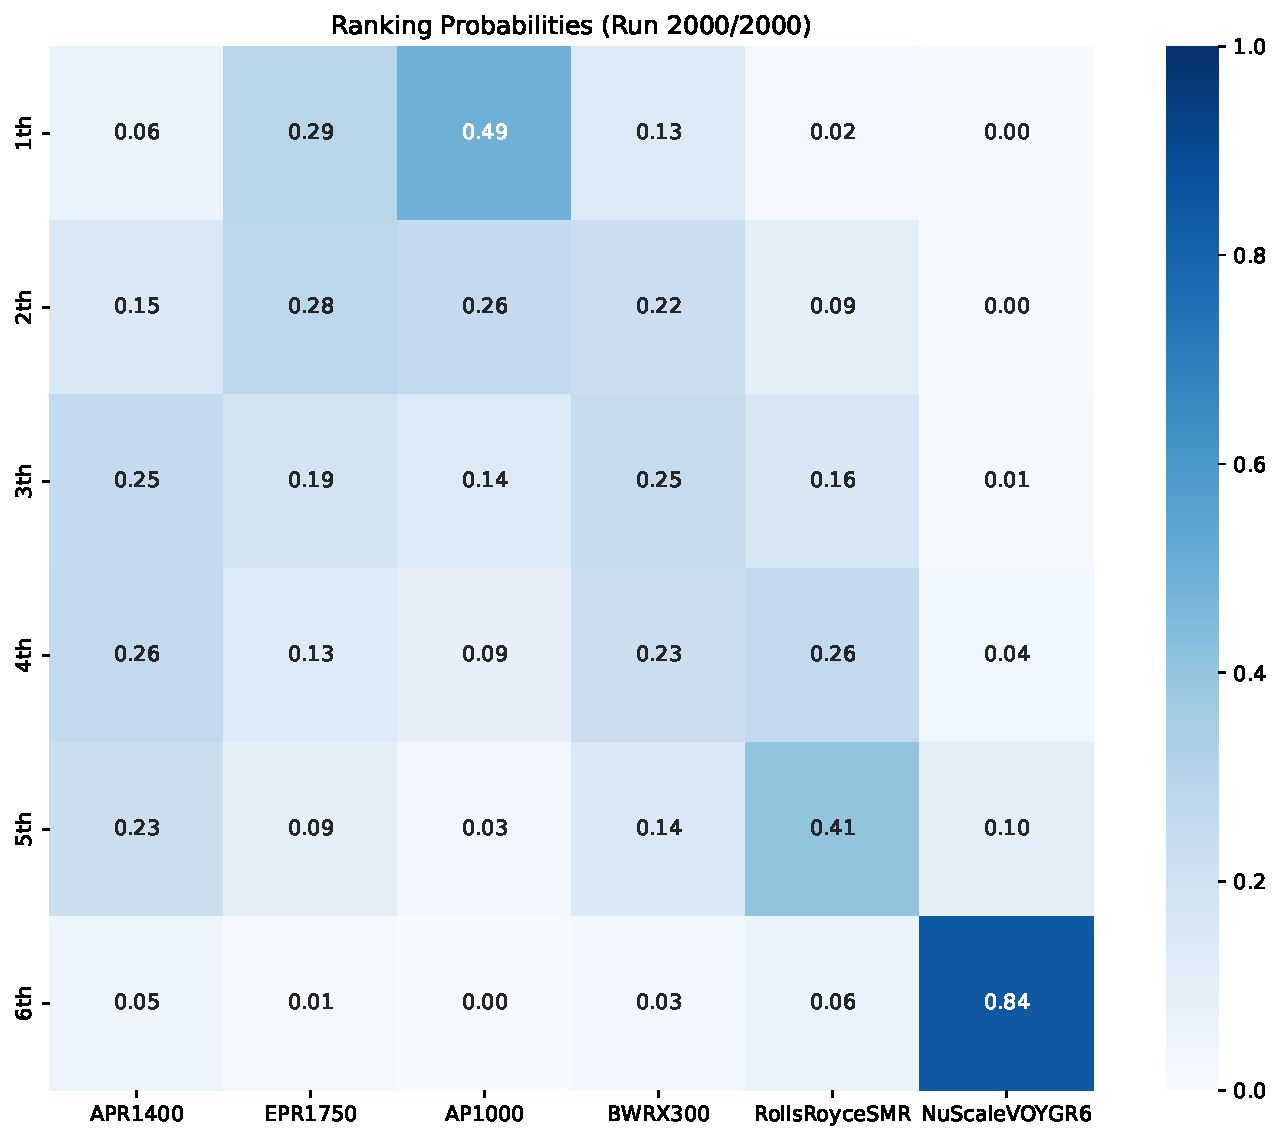
\includegraphics[width=0.45\linewidth]{Phase3_AllMethods_CH_geometric_mean_20260127_172000_heatmap.pdf}}\hfill
	\subfloat[France]{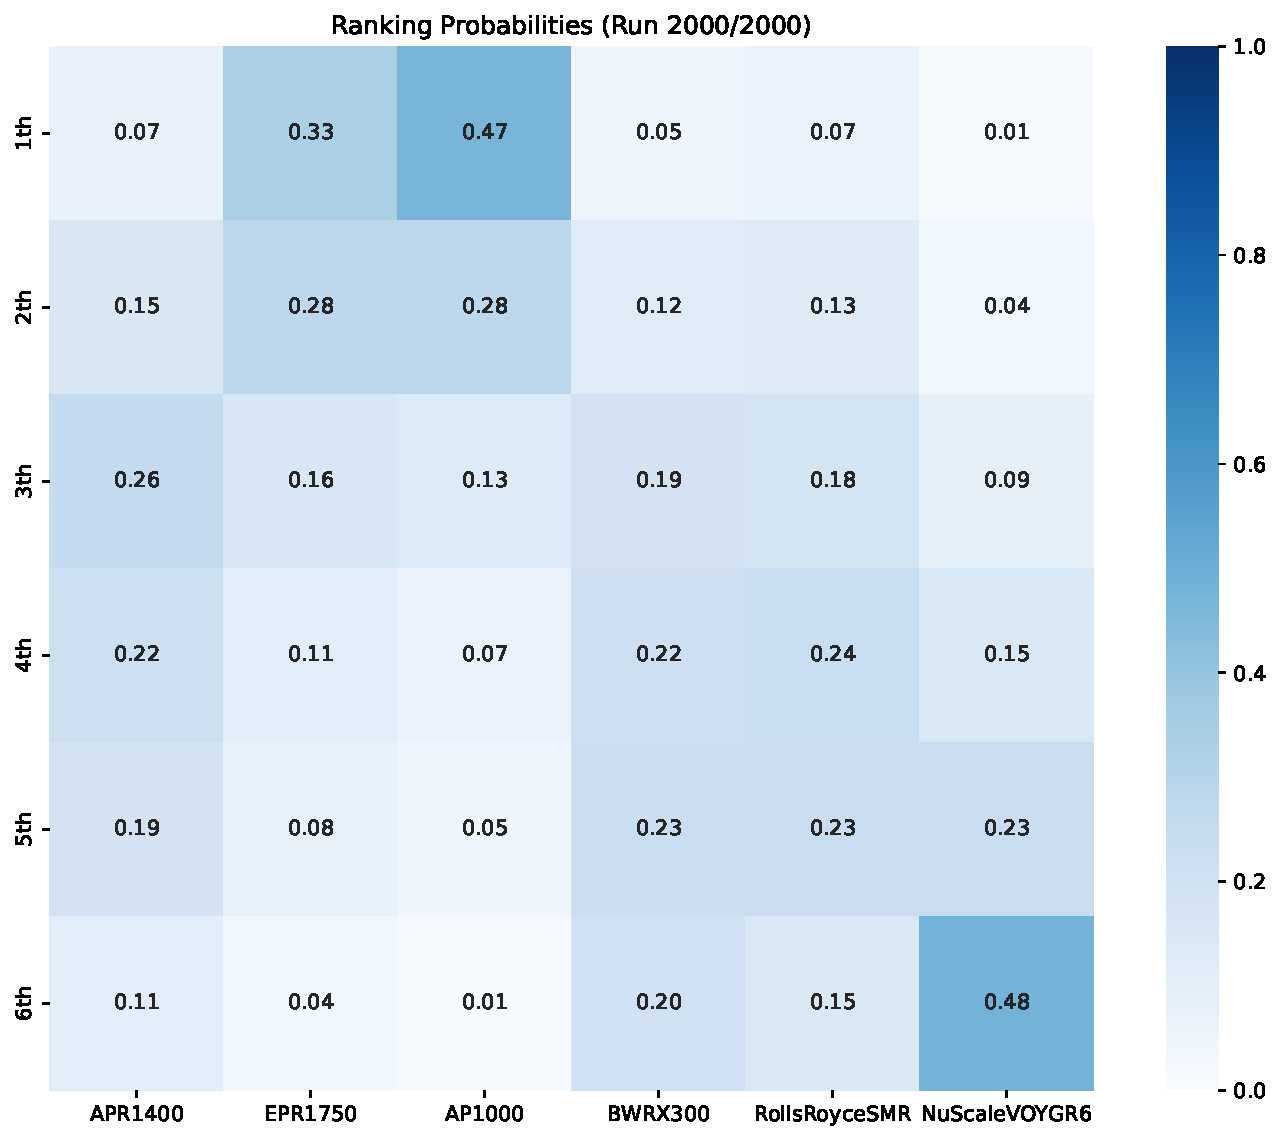
\includegraphics[width=0.45\linewidth]{Phase3_AllMethods_FR_geometric_mean_20260127_171648_heatmap.pdf}}
	\caption{NSMC ranking heatmaps (geometric mean) for Switzerland and France. Columns represent alternatives and rows ranking tiers. The preference for large reactors is consistent across national contexts.}
	\label{fig:nsmc_ch_fr}
\end{figure}

Subtle national variations appeared in the lower rankings: Italy and Poland both favoured the Rolls-Royce SMR among smaller designs, while France and Switzerland demonstrated a preference for the BWRX-300. These differences remained confined to secondary alternatives, suggesting overall consistent preferences across Western European contexts.

\subsection{Consensus and Uncertainty Analysis}

The Strict Monte Carlo (SMC) output shows high consensus on alternative values, though the BWRX-300 and Rolls-Royce SMR showed greater divergence, with the former exhibiting two distinct probability peaks. When applying geometric mean aggregation, lower-ranked alternatives displayed narrow, low-value distributions, such as those in Figure~\ref{fig:nuscale_poland}, enabling confident elimination of these low performing alternatives. In contrast, top alternatives (EPR, AP1000) produced broader, flatter distributions, indicating higher decision uncertainty, see Figure~\ref{fig:ap1000_poland}. Among these, the AP1000 presented the lowest risk profile, as it was the only top contender without a rising probability toward lower performance values.

Capital investment costs, supplier availability, and complexity indicators emerged as universally critical criteria, while load-following capabilities were largely dismissed. Technical parameters (thermal efficiency, discharge burnup) were consistently deemed irrelevant from a policy perspective.

\begin{figure}[htbp]
    \centering
    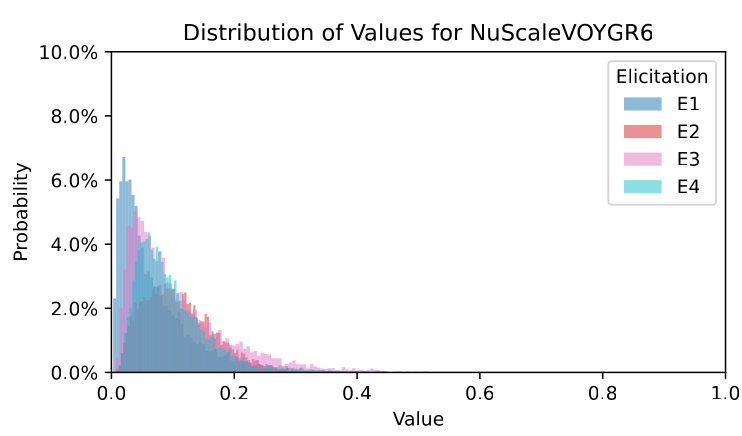
\includegraphics[width=0.95\linewidth]{bad_performing_example.png}
    \caption{SMC output for Nuscale alternative in Poland (geometric mean).}
    \label{fig:nuscale_poland}
\end{figure}


\begin{figure}[htbp]
    \centering
    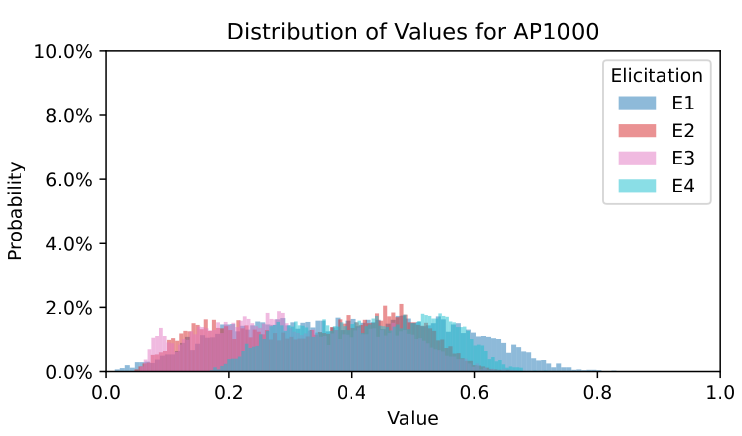
\includegraphics[width=0.95\linewidth]{good_performing_example.png}
    \caption{SMC output for AP1000 alternative in Poland (geometric mean).}
    \label{fig:ap1000_poland}
\end{figure}


\subsection{Policy Implications}

The observed preference for large reactors requires scrutiny in light of long-term grid stability. As European grids integrate higher shares of variable renewable energy, low-flexibility solutions risk becoming a liability. Policymakers should therefore adopt a pan-European perspective when planning nuclear expansions, prioritizing metrics that capture cross-border interdependencies and balanced deployment strategies, transcending national contexts for the sake of grid stability and resilience.

%-----------------------------------------------------------------------------
% CONCLUSIONS
%-----------------------------------------------------------------------------
\section{Conclusions}
\label{sec:conclusions}
This thesis developed and applied the UP-MAVT framework to a case study comparing reactor designs across multiple European countries, producing and interpreting results under deep uncertainty. The key contributions of this study are:
\begin{enumerate}
    \item \textbf{The UP-MAVT framework} itself, which propagates uncertainties from quantitative and qualitative data, value functions, and weights simultaneously using Monte Carlo method, providing full probability distributions rather than point estimates or ranges.
    \item \textbf{Open-source digital tools} for interactive elicitation of value functions, qualitative indicators, and weights with real-time consistency checking.
    \item \textbf{A novel case study} comparing reactor designs across multiple European countries, revealing a consistent expert preference for large reactors over SMRs in grid deployment, driven primarily by feasibility and politcal factors rather than technical performance.
\end{enumerate}

Future work should refine the case study by selecting a specific deployment site, enabling the integration of site-dependent social and environmental indicators. The framework could be strengthened through detailed uncertainty tracking to map origins and propagation pathways, while methodological expansions might explore outranking MCDA approaches. To broaden expert participation, remote, self-paced elicitation tools should also be developed.

%-----------------------------------------------------------------------------
% ACKNOWLEDGEMENTS
%-----------------------------------------------------------------------------
\section*{Acknowledgements}
This work has been partially supported by the ENEN2plus project (HORIZON-EURATOM-2021-NRT-01-13 101061677) funded by the European Union.

%---------------------------------------------------------------------------
%  BIBLIOGRAPHY
%---------------------------------------------------------------------------
\bibliography{bibliography.bib}

\begin{figure*}[p]
    \centering
    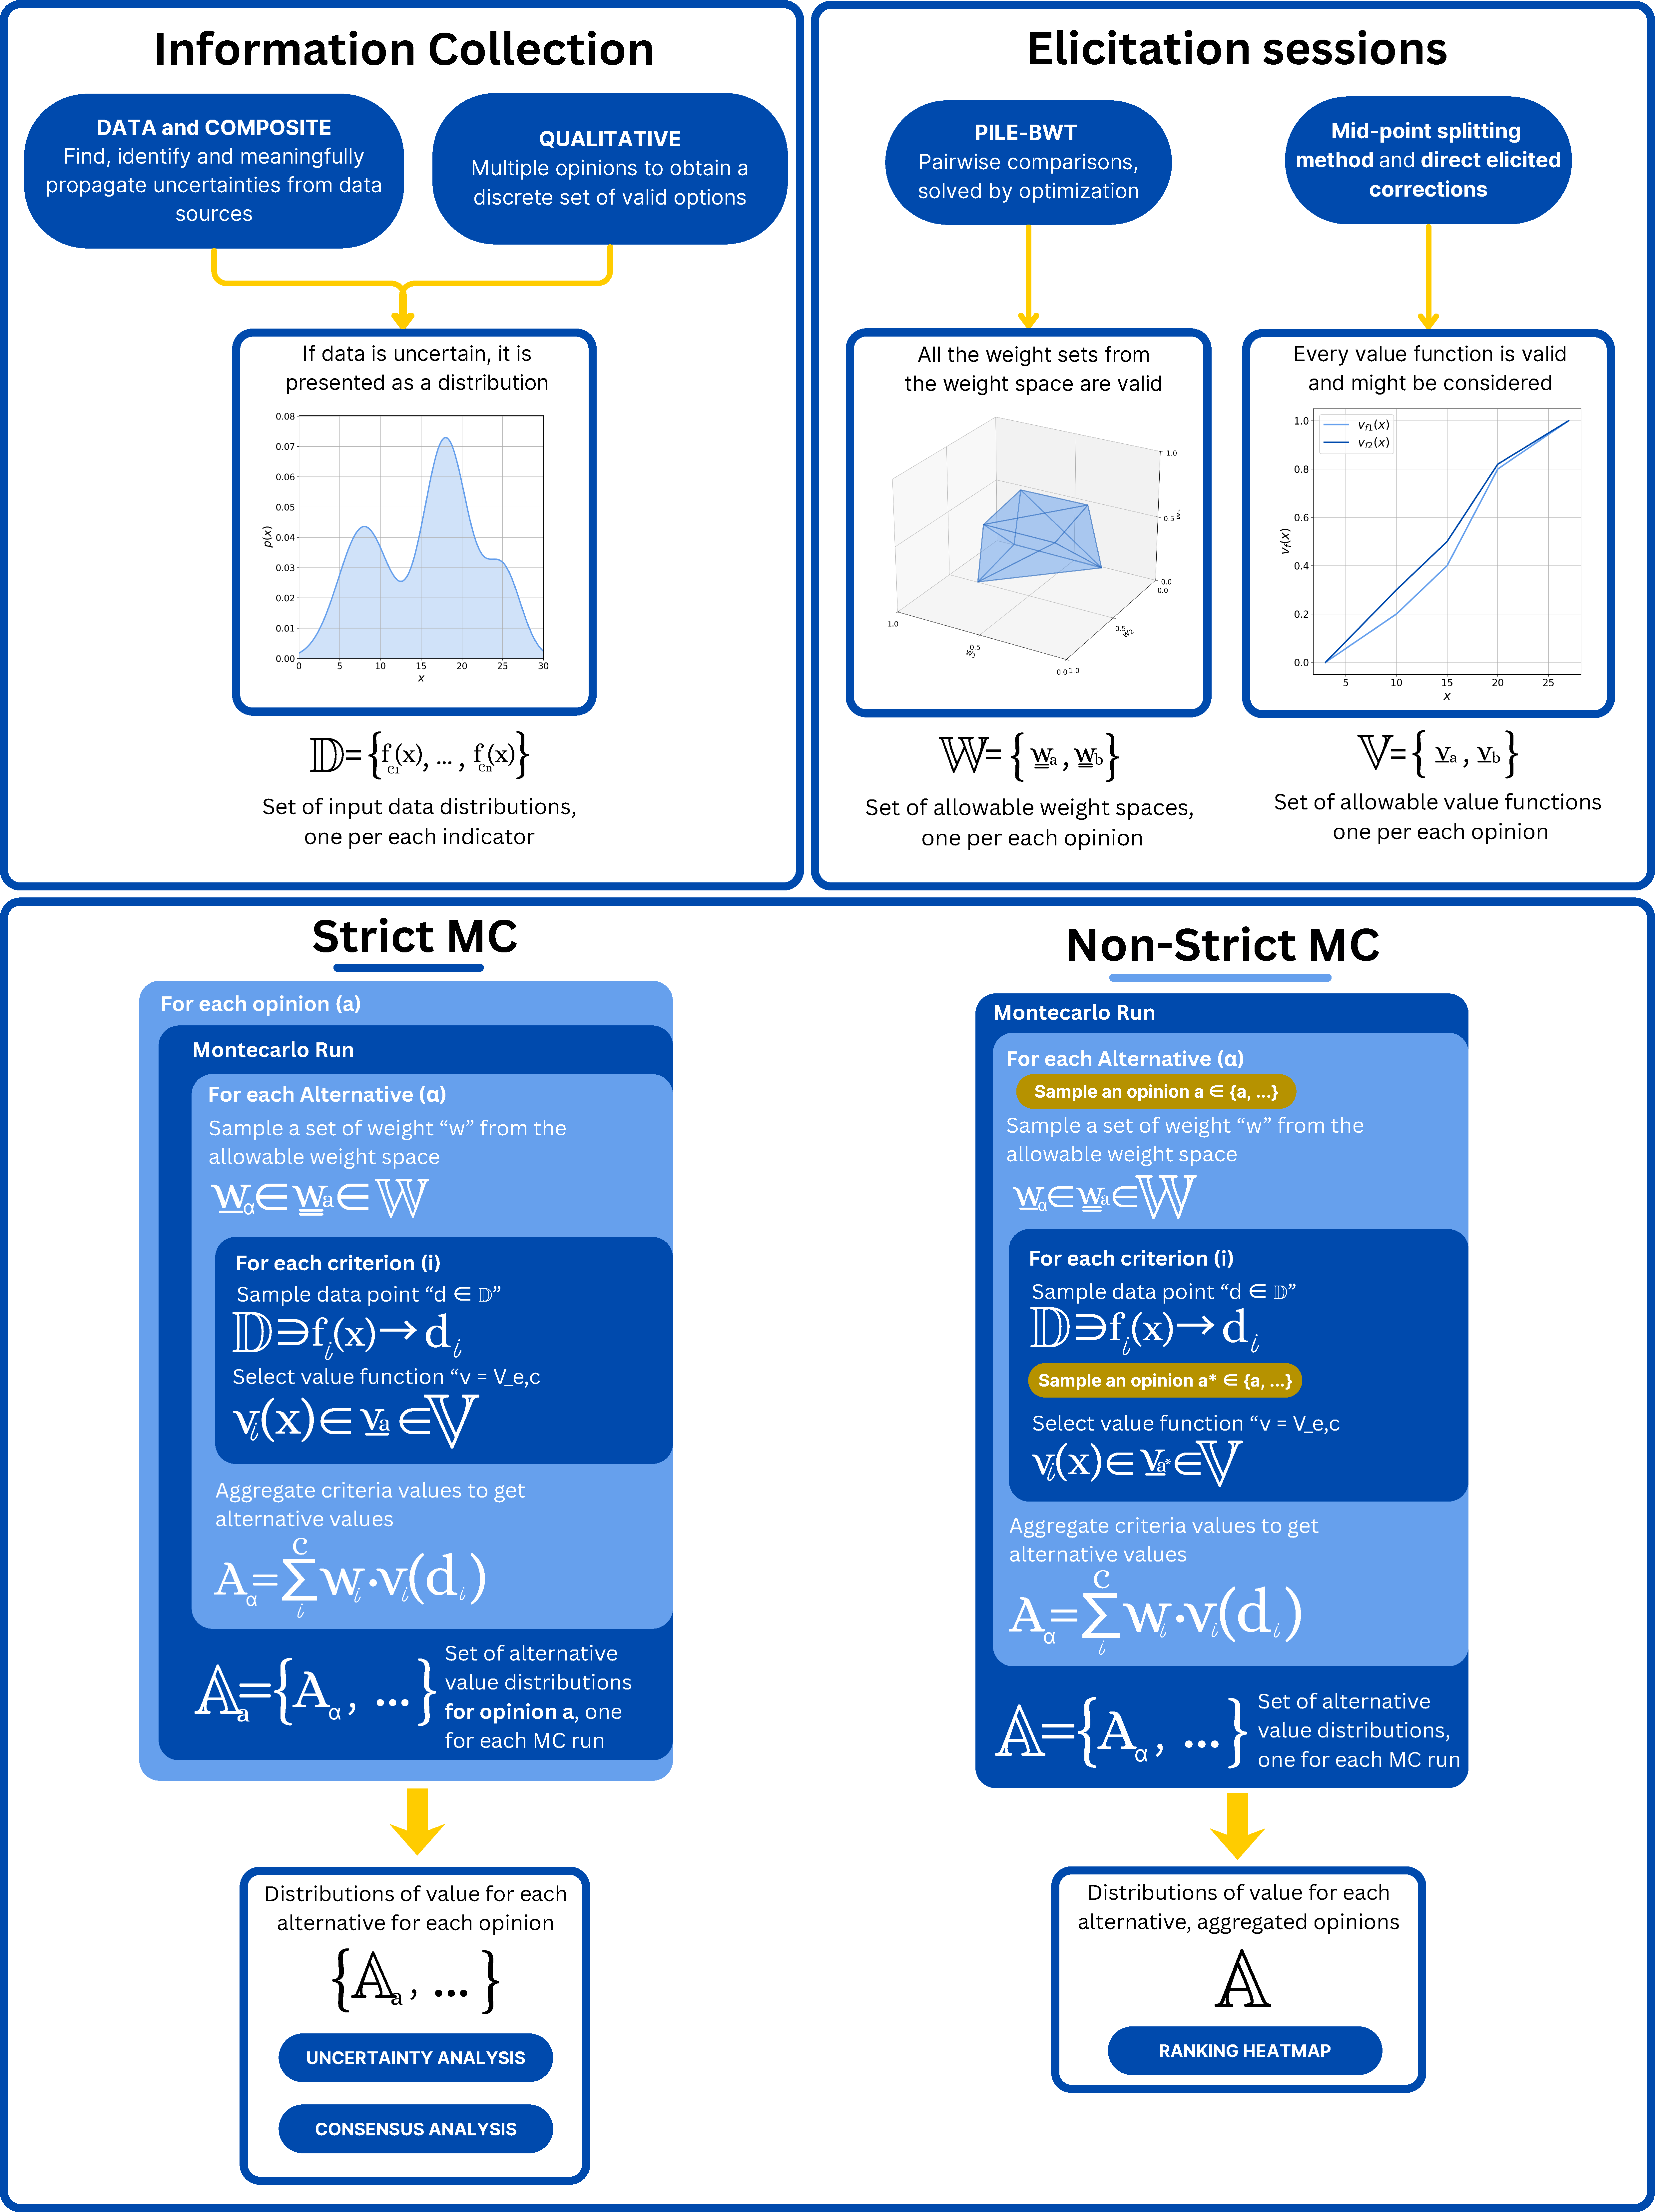
\includegraphics[width=0.95\textwidth]{UP-MAVT_workflow.pdf}
    \caption{UP-MAVT workflow: sources of uncertainty in data and elicitation results are propagated through Monte Carlo simulation to produce probabilistic rankings.}
    \label{fig:workflow}
\end{figure*}

\end{document}